In this chapter we present the results relevant to our discussed topics in the 
next chapter. To keep this chapter structured in a way that makes it easy to 
look up we divide our results into five main sections presenting model importance 
and feature importance for four cases:
\begin{enumerate}
    \item Models trained on CAMELS-GB \citep{CAMELS_GB}.
    \item Models trained on CAMELS \citep{CAMELS_US} in additiion to traditional 
        models provided by \citationneeded.
    \item Models trained on a dataset comprised of both CAMELS and CAMELS-GB.
    \item Models trained on CAMELS and validated on CAMELS-GB and vice-versa.
    \item Models refit on the full train set and valiated on the test set not 
        touched in sections 1 - 4.
\end{enumerate}

\section{Models trained on CAMELS-GB}
In this section we present the results related to model selection and feature 
importance when training and predicting on CAMELS-GB \citep{CAMELS_GB}. To act 
as a proof of concept of the feature importance method described in Chapter 
\ref{Feature selection} we also include the performance and feature importance of 
a model trained using dataset a (see Table \ref{attribute table}) in addition to
static attributes directly derived from the observed outcome.

\subsection{Performance}
\begin{figure}
    \centering
    \includegraphics{{results_section/camels_gb/cdf_val}.pdf}
    \caption{Cumulative distribution function of the NSE score of LSTM models trained 
    on CAMELS-GB \citep{CAMELS_GB}. "Overfit model" is a model deliberately trained 
    using static basin attributes derived from the runoff time series of the basins. 
    The other models are described in Table \ref{all models}.}
    \label{CAMELS-GB CDF validation}
\end{figure}
Figure \ref{CAMELS-GB CDF validation} shows the performance of several LSTM models 
trained on CAMELS-GB \citep{CAMELS_GB}. The overfit model is trained on dataset a 
in Table \ref{attribute table} in addition to attributes directly derived from the 
observed outcome.
The overfit model significantly outperforms all other models.
 Of the other models there seems to be generally two levels of 
performance. The models using attribute subsets a and b perform similarly, although 
in the favour of dataset a, while 
the models trained with no attributes in general perform worse. Enabling dropout 
slightly decreases performance.
There seems to be little overall difference in performance between EA-LSTM and 
LSTM models, apart from $GB_{lstm, all}$ which performs with a negative NSE value 
for a smaller fraction of the basins.
 All other ungauged  models perform with a negative NSE value for 
approximately 10\% of the basins.

\subsection{Importance}
\section{Models trained on CAMELS}
In this section we present the results related to model selection and feature 
importance when training and predicting on CAMELS \citep{CAMELS_US}. This section 
is meant to show whether we are able to produce results similar to the those of 
\citet{lstm_third_paper} in a way that is comparable to the rest of our experiments.
In addition we present apparent feature importance of these trained models.
\subsection{Performance}
\begin{figure}
    \centering
    \includegraphics{{results_section/camels_us/cdf_val}.pdf}
    \caption{Cumulative distribution function of the NSE score of models trained 
    on CAMELS \citep{CAMELS_US}. "VIC" is the Variable Infiltration Capacity model 
    calibrated on CAMELS. "SAC-SMA" is the SACramento Soil Moisture Accounting 
    model calibrated on CAMELS. 
    These benchmarks are provided by \citet{CAMELS_hydroshare} and are originally 
    created by \citet{VICbench} and are trained per-basin as opposed to the other 
    models.
    "NWM" is a benchmark of the National Water Model run on CAMELS. (CHECK IF PER-BASIN, 
    I THINK ITS UNGAUGED!!!). This benchmark is available without any licensing at 
    \citet{NWMbench} and we use an already preprocessed version provided by 
    \citet{lstm_third_paper}.
    The other models are described in Table \ref{all models} and are based on the 
    models originally trained by \citet{lstm_third_paper} but retrained for better 
    comparison with the other LSTM models in this thesis.}
    \label{CAMELS-US CDF validation}
\end{figure}
Figure \ref{CAMELS-US CDF validation} shows the performance of our reimplementation 
of the model created by \citet{lstm_third_paper} along with three traditional 
hydrological models. The results here indicate that the process-driven models 
VIC and NWM perform similarly, SAC-SMA and an LSTM without basin attributes perform 
similarly and better than the process-driven model and that there is a clear difference 
in performance in favour of US$_\text{Kratzert}$. The LSTM models both perform 
with an NSE value below zero for approximately five percent of the basins used 
for validation. 
\subsection{Importance}
\section{Models trained on CAMELS and CAMELS-GB}
In this section we present results related to model selection and feature importance 
when training and validating using both CAMELS and CAMELS-GB as a combined dataset.
This section is meant to show whether we can obtain satisfactory performance on 
ungauged basins from both datasets with the same model. 

\subsection{Performance}
\begin{figure}
    \centering
    \includegraphics{{results_section/mixed/cdf_val}.pdf}
    \caption{Cumulative distribution function of the NSE score of LSTM models trained 
    on a dataset consisting of both CAMELS \citet{CAMELS_US} and CAMELS-GB \citep{CAMELS_GB}. 
    The models are described in Table \ref{all models}. The top figure shows the 
    performance of the models on CAMELS-GB and the bottom figure shows the performance 
    on CAMELS. The top figure is the cross validated perforamnce on CAMELS-GB, the 
    bottom figure on CAMELS.}
    \label{mixed CDF validation}
\end{figure}
Figure \ref{mixed CDF validation} shows the cross validated performance of three 
LSTM models trained on a dataset consisting of both CAMELS and CAMELS-GB. 
On CAMELS-GB the models with basin attributes perform significantly better than 
the model trained without them. This also applies to the performance on CAMELS, 
but here the difference is smaller. The EA-LSTM and LSTM models with basin attributes 
perform similarly, having a median NSE of $~0.77$ on CAMELS-GB and $~0.65$ on CAMELS.
Compared to the best performing models in Figure \ref{CAMELS-GB CDF validation} and \ref{CAMELS-US CDF validation} 
the performance of the mixed model is comparable, although lower.
\subsection{Importance}
\section{Models trained for transfer learning between CAMELS and CAMELS-GB}
In this section we present results related to model selection and feature importance 
when training on CAMELS-GB and validating on CAMELS and vice-versa. This section 
is meant to show whether we can use information in one dataset to be able to 
satisfyingly make predictions on the other.
\subsection{Performance}
\begin{figure}
    \centering
    \includegraphics{{results_section/transfer/cdf_val}.pdf}
    \caption{Cumulative distribution function of the NSE score of LSTM models trained 
    on CAMELS \citep{CAMELS_US} and validated on a validation part of CAMELS as well as 
    the entirety of CAMELS-GB \citep{CAMELS_GB}. The top figure shows the 
    performance of the models on CAMELS-GB and the bottom figure shows the performance 
    on CAMELS.}
    \label{transfer CDF validation}
\end{figure}
\begin{figure}
\includegraphics{{results_section/transfer/training_progress}.pdf}
\caption{Training performance per epoch of Transfer$_\text{US, none}$ and Transfer$_\text{GB, none}$ 
on CAMELS-GB (top) and CAMELS (bottom). The orange line indicates the median NSE, 
the green line indicates the mean NSE.}
\label{training progress transfer}
\end{figure}
Figure \ref{transfer CDF validation} shows models trained on CAMELS and validated on 
CAMELS-GB and vice-versa. No models trained on CAMELS-GB perform at a satisfactory level 
on basins from CAMELS. The models trained on CAMELS all perform at a lower level 
on CAMELS-GB than models that are trained on CAMELS-GB and the best performing 
transfer model is Transfer$_\text{US, none}$. This model has no access to static 
basin attributes. The transfer models also perform worse on the validation part of 
the dataset they are trained on as the chosen epoch is based on the performance 
on both datasets. This is illustrated in Figure \ref{training progress transfer}, 
which shows boxplots of the performance per epoch of Transfer$_\text{US, none}$ and Transfer$_\text{GB, none}$ 
per training epoch on both CAMELS-GB (top) and CAMELS (bottom). We observe that 
the performance of Transfer$_\text{US, none}$ increases on CAMELS-GB up until 
epoch 5 and then gradually decreases while it increases steadily and converges 
on CAMELS around epoch 10. The epoch optimized for both datasets which is shown in 
Figure \ref{transfer CDF validation} is epoch 9. For Transfer$_\text{GB, none}$ 
this is more apparent. Epoch 1 is the best epoch for the performance on CAMELS, 
while the performance on CAMELS-GB seems to increase for every epoch. The optimized 
epoch found for this model is epoch 24.
\subsection{Importance}
\section{Test performance of best models}
\begin{figure}
\centering
\includegraphics{{results_section/camels_gb/cdf_test}.pdf}
\caption{Something something test results}
\label{test gb}
\end{figure}
In this section we present test results from the models we choose from Section 1 - 4 
in this chapter and compare to the validation performance.
%\begin{table}
%    \begin{adjustbox}{width=\textwidth}
%    \begin{tabular}{lr}
\toprule
{} &     Coeff \\
\midrule
Q95                   &  1.211018 \\
elev\_50               &  0.464968 \\
conductivity\_cosby\_50 &  0.443736 \\
intercept             &  0.443277 \\
porosity\_cosby\_50     &  0.409635 \\
conductivity\_hypres\_5 &  0.257509 \\
high\_prec\_dur         &  0.211253 \\
gauge\_easting         & -0.211231 \\
tawc                  & -0.326509 \\
elev\_max              & -0.349975 \\
conductivity\_cosby\_5  & -0.351292 \\
baseflow\_index\_ceh    & -0.417237 \\
bares\_perc            & -0.463398 \\
elev\_10               & -0.496951 \\
conductivity\_cosby\_95 & -0.839606 \\
porosity\_hypres\_5     & -1.030274 \\
low\_prec\_freq         & -1.055273 \\
dwood\_perc            & -1.288324 \\
p\_mean                & -2.015090 \\
ewood\_perc            & -2.146395 \\
urban\_perc            & -2.332153 \\
shrub\_perc            & -3.735298 \\
grass\_perc            & -4.010000 \\
crop\_perc             & -4.868455 \\
\bottomrule
\end{tabular}


%    \end{adjustbox}
%    \caption{Table for attempt at linear regression. This model is fit on the static
%    features as input values, and the NSE of an LSTM trained without static features
%    for each basin in the validation set. The $R^2$ score of this model is $\approx 0.5$}
%    \label{linreg_no_static_table}
%\end{table}
%In table \ref{linreg_no_static_table} we can see that our linear regression used to model 
%the relationship between NSE value of models and static features has decided that 
%several features are important. All these coefficients have a p-value $<0.5$. The 
%problem with this model was that it achieved an $R^2$ score of $\approx 0.5$, meaning 
%it does not actually explain the relationship well. We therefore choose to change 
%strategy for feature selection. 
\begin{comment}
\begin{figure}
    \includegraphics{{correlation_reduction/all_features/corr_and_dendrogram}.pdf}
    \caption{The Pearson correlation matrix and the corresponding hierarchial
    cluster of the training set before removing correlated features. The process
    of creating the dendrogram is described in chapter \ref{Feature selection}. 
    For readability's sake we cannot include every label in the correlation matrix.}
    \label{corr_matrix_full}
\end{figure}

\begin{figure}
    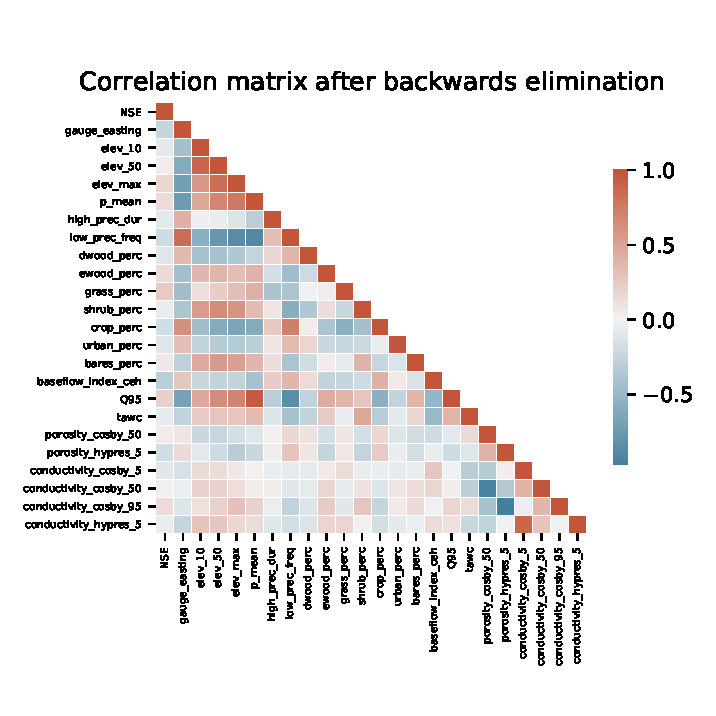
\includegraphics{reduced_matrix.pdf}
    \caption{Correlation matrix after backward selection}
    \label{corr_matrix_reduced}
\end{figure}

%\subsection{Performance of full model}
\begin{figure}
%\includegraphics[scale=1]{{permutation/all_features_cv/histogram_all}.pdf}
    \includegraphics{{figures/permutation/all_features_cv/histogram_all}.pdf}
\caption{The two most important (above) and least important (below) features according 
to the permutation test}
\label{Hist all}
\end{figure}



\begin{figure}
    \centering
    \includegraphics{{CDFs/mixed_model_comparisons}.pdf}
    \caption{top kjeks}
    \label{main cdf}
\end{figure}
\end{comment}
